\documentclass{../exercisesheet}

\title{Datenkommunikation und Informationssysteme, Übung 8}
\author{
    Domenic Quirl \\ 354437
    \and
    Julian Schakib \\ 353889
    \and 
    Daniel Schleiz \\ 356092
}

\renewcommand{\Exercise}{Aufgabe}
\date{Übungsgruppe 14}

\usepackage{float}
%\usepackage{siunitx}
\usepackage{color}
\usepackage{multirow}
\usepackage{float}

\begin{document}
\maketitle
\pointtable


\begin{exercise}{6}
\begin{subexercise}
\begin{center}
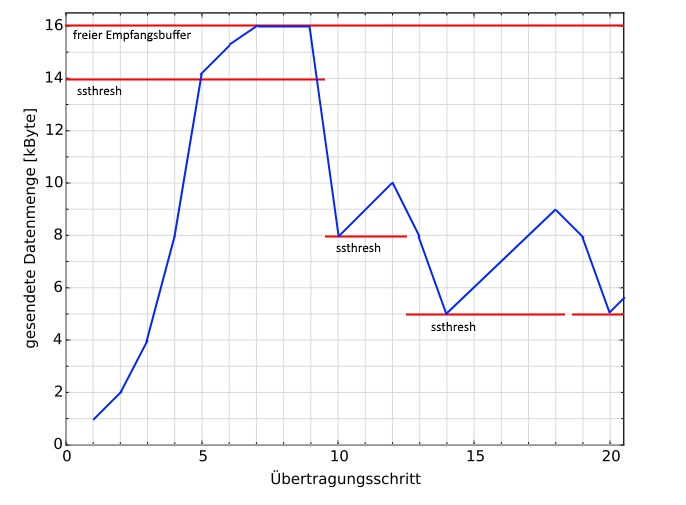
\includegraphics[scale=0.8]{1a.jpg}
\end{center}
\end{subexercise}
\begin{subexercise}
\begin{description}
\item[i)] \ \\
Da es keine Übertragungsfehler gibt, wächst das \textbf{cwnd} bei \textbf{ssthresh}=32 kByte wie folgt:
\begin{center}
\begin{tabular}{c||*{7}{c|}c}
Übertragungsschritt & 1 & 2 & 3 & 4 & 5 & 6 & 7 & 8\\
\hline
\textbf{cwnd} & 1 & 2 & 4 & 8 & 16 & 32 & 33 & 34\\
\end{tabular}
\end{center}
Betrachtet man nur die Restriktionen des \textbf{cwnd}, hätte man so insgesamt 130 kByte übertragen können. Das anfängliche \textbf{rwnd} beträgt allerdings nur 128 kByte, sodass, falls in der Zwischenzeit nichts aus dem Buffer ausgelesen wird, auch nur 128 kByte übertragen werden können. Werden 1 oder 2 kByte gelesen, so können 129 bzw. 130 kByte übertragen werden.
\item[ii)] \ \\
Die Übertragungsrate hängt davon ab, wie schnell die Daten beim Empfänger aus dem Buffer gelesen werden. Da keine Übertragungsfehler auftreten, kann mit genügend Zeit das \textbf{cwnd} bis auf 128 oder mehr steigen, es können also in einem Schritt 128 kByte gesendet werden. Wenn wir davon ausgehen, dass eingehende Segmente sofort aus dem Buffer gelesen werden, bevor das nächste Segment eintrifft, so werden sie jeweils mit einer Restgröße des Buffers von 127 kByte bestätigt, sodass in jedem Schritt (pro 40ms) 127 kByte gesendet werden können. Dies ergibt sich zu 3175 kByte/s.

Geht man hingegen davon aus, dass der Buffer immer nur zwischen zwei Übertragungsschritten gelesen wird, so lassen sich maximal 128 kByte alle zwei Schritte übertragen, mit einem Schritt dazwischen, in dem aufgrund des zuletzt als voll bekannten Buffers nicht gesendet wird (außer eventuell 1 Segment aufgrund des Persistence Timers, aber dies würde dann das Fenster im nächsten Schritt auch um 1 verkleinern). So erreicht man 128 kByte pro 80ms, welches sich zu 1,6 MByte/s ergibt. Dies ist äquivalent zu einer beliebigen Aufteilung der 128 kByte auf zwei Schritte, zwischen denen jeweils der Buffer komplett ausgelesen wird, z.B. 2 * 64 kByte.
\end{description}
\end{subexercise}
\begin{subexercise}
Die Idee der DUP-ACKs ist, auszugleichen, dass Pakete nicht garantiert in der richtigen Reihenfolge ankommen, da TCP mit IP arbeitet. Wenn man also direkt auf das erste DUP-ACK reagieren würde, welches gesendet wird, wenn ein Paket mit falscher Sequenznummer ankommt, würde man die Übertragung wiederholen, sobald ein Paket nicht in der richtigen Reihenfolge ankommt, also gerade nicht das, was man erreichen will. Stattdessen erlaubt man bis zu zwei anderen Paketen, welche eigentlich nach dem nächsten erwarteten Paket liegen, vor diesem anzukommen, und erst beim dritten wird die Übertragung wiederholt. 
\end{subexercise}
\end{exercise}


\begin{exercise}{4}
\begin{subexercise}
\begin{description}
\item[i)] Bei einen passiven Angreifer bleibt der Diffie-Hellman Schlüsselaustausch sicher. Der Angreifer hat keine Kenntnis über die jeweils zufällig gewählten Zahlen $S_A$ und $S_B$
von Alice und Bob und ist auch nicht in der Lage, Nachrichten zu manipulieren. Aufgrunddessen kann der Angreifer den Schlüssel $g^{S_A \cdot S_B} \text{ mod } p$ nur herausfinden, 
indem er $S_A$ und $S_B$ durch diskretes Logarithmen von $T_A=g^{S_A} \text{ mod }p$ und $T_B$ berechnet. Dies ist jedoch nicht effizient möglich, weshalb auch die Berechnung
des Schlüssels nicht effizient möglich ist.

\item[ii)] Bei einem aktiven Angreifer ist der Diffie-Hellman Schlüsselaustausch nicht mehr sicher. Da Pakete manipuliert werden können, kann der Angreifer sich selber eine gültige Zufallszahl
$S_M$ generieren und jeweils die Übertragung von $T_A$ und $T_B$ stoppen und an dessen Stelle $T_M=g^{S_M} \text{ mod }p$ weiterleiten. $A$ und $B$ besitzen jeweils
unterschiedliche Schlüssel $K_1=T_M^{S_A}=g^{S_M \cdot S_A} \text{ mod }p$ und $T_M^{S_B}=g^{S_M \cdot S_B} \text{ mod }p$, jedoch ist es für den Angreifer möglich, unter Kenntnis
von $S_M$, $K_1$ und $K_2$ zu berechnen.
\end{description}
\end{subexercise}
\begin{subexercise}
Alice berechnet $T_A=3^3 \equiv_{17} 10$ und übertragt diese Zahl an Bob, während Bob $T_B=3^2 \equiv_{17} 9$ berechnet und dies an Alice überträgt.
Nun berechnen Alice und Bob $T_B^{S_A}$ bzw. $T_A^{S_B}$, was in beiden Fällen gleich $3^{S_A \cdot S_B} = 3^6 = 3^3 \cdot 3^3 \equiv_{17} 10 \cdot 10 \equiv_{17} 15$.
Also ist der (symmetrische) Schlüssel bestimmt durch 15.
\end{subexercise}
\end{exercise}


\begin{exercise}{5}
\begin{subexercise}
Da $p=13$ und $q=23$, ist $n=p\cdot q = 299$. Der public key ist also $\langle 61,299 \rangle$. Zudem ist $\Phi(299)=(13-1)\cdot(23-1)= 264$. Finde nun $d$ so, dass
$d \cdot e = d \cdot 61 \equiv_{264} 1$. Verwende den erweiterten Algorithmus von \textsc{Euklid}:
\begin{align*}
264 &= 4 \cdot 61 + 20	&	1&=61-3\cdot 20 \\
61 &= 3 \cdot 20 + 1	&	 &= 61-3 \cdot(264-4\cdot 61) \\
20 &= 20 \cdot 1 + 0	&	 &= -3 \cdot 264 + 13 \cdot 61 \\
\null &				&	 &\equiv_{264} 13 \cdot 61
\end{align*}
Nun folgt also, dass der private key $\langle 13, 299 \rangle$ ist.
\begin{itemize}
\item Verschlüssele $m_1=21$: $c_1 = 21^{61} \equiv_{299} 281$.
\item Entschlüssele $c_2=291$: $m_2=291^{13} \equiv_{299} 5$.
\end{itemize}
\end{subexercise}
\begin{subexercise}
Es ist bekannt, dass $n=91$. Finde durch geschicktes Ausprobieren heraus, dass die Primfaktorzerlegung von $n$ gegeben ist durch $p=7$, $q=13$, da $91 = 7 \cdot 13$.
Außerdem ist $\Phi(n)=6 \cdot 12 = 72$. Suche nun $d$, sodass $d \cdot e= d \cdot 29 \equiv_{72} 1$. Verwende erneut den erweiterten Algorithmus von \textsc{Euklid}:
\begin{align*}
72 &= 2 \cdot 29 + 14	&	1 &= 29 - 2 \cdot 14 \\
29 &= 2 \cdot 14 + 1	&	  &= 29 - 2 \cdot (72-2 \cdot 29) \\
14 &= 14 \cdot 1 + 0	&	  &= -2 \cdot 72 + 5 \cdot 29 \\
\null &				&	  &\equiv_{72} 5 \cdot 29
\end{align*}
Es folgt, dass der private key gegeben ist durch $\langle 5,91\rangle$.
\begin{itemize}
\item Dekodiere $c=3$ zu $m=3^5 \equiv_{91} 61$.
\end{itemize}
\end{subexercise}
\end{exercise}



\end{document}

